\chapter{Uživatelská dokumentace}
Platforma je uživateli přístupná pomocí dvou aplikací -- grafického a textového
rozhraní. Funkčnost aplikací byla otestována na operačních systémech Windows
a~Linux. Všechny aplikace jsou vytvořené v jazyce Python a tedy všechny soubory
mají přípony \emph{.py}. 

Uživatelskou dokumentaci rozdělíme do dvou částí. V první v části
\ref{doc_1_spust_a_kompon} si popíšeme kroky potřebné ke spuštění aplikací a
předvedeme jednotlivá rozhraní a~práci s nimi. V druhé části
\ref{doc_2_experimenty} si poté předvedeme jak se pomocí těchto rozhraní tvoří
a provádějí experimenty.

\section{Spuštění a komponenty rozhraní} \label{doc_1_spust_a_kompon}

V této sekci se nejprve podíváme jak připravit prostředí se všemi potřebnými
knihovnami pro správné fungování celé platformy (v podsekci
\ref{doc_11_spust}). Dále si předvedeme uživatelská rozhraní -- grafické v
podsekci \ref{doc_12_GUI} a poté textové v~podsekci~\ref{doc_13_TUI}.

\subsection{Instalace a spuštění rozhraní} \label{doc_11_spust}
Celá platforma je vytvořená za pomoci několika knihoven, které musí být před
spuštěním nainstalované pro zajištění správné funkčnosti všech aplikací. Pro
usnadnění instalace všech potřebných knihoven bylo pomocí prostředí pro správu
balíčků \href{https://conda.org/}{\emph{Conda}} vytvořené vlastní prostředí, ve
kterém aplikace poběží. 

\paragraph{Instalace \emph{Conda}}

Uživatel nejprve musí nainstalovat \emph{Condu}. K tomu můžeme využít
minimalistický instalátor \emph{Miniconda} (dostupný na všech platformách
z~oficiálních stránek \url{https://docs.conda.io/en/latest/miniconda.html}).

Po stažení a instalaci tohoto instalátoru by měl uživatel mít z příkazové řádky
(popřípadě s využitím specializované \emph{Conda} příkazové řádky)) přístup k
příkazu \texttt{conda}, který umožňuje ovládat prostředí pro správu balíčků. 

\paragraph{Tvorba prostředí}
Nyní můžeme v kořenové složce této práce využít následujícího příkazu pro
tvorbu prostředí pro naši aplikaci.
\begin{code}
conda env create -f conda_environment/environment.yml
\end{code}
Tento příkaz je volán přes příkaz \texttt{conda}. Pomocí spojení \texttt{env
create} specifikujeme, že chceme vytvářet nové prostředí pro běh aplikací.
Parameter \texttt{-f} příkazu říká, že bude následovat vstupní soubor (cesta ke
konfigurarčnímu souboru), pomocí kterého má být prostředí vytvořeno. Tento
konfigurační soubor se jménem \emph{environment.yml} je z pohledu kořenového
adresáře umístěn ve složce \emph{conda\_environment}.

Konfigurační soubor specifikuje detaily prostředí, jako jeho jméno (v našem
případě \emph{roboEvo}) a balíčky, které má nainstalovat.

Po doběhnutí instalace prostředí může být prostředí aktivováno pomocí příkazu
\texttt{conda activate roboEvo} a poté deaktivováno pomocí \texttt{conda
deactivate}. Pokud máme aktivované prostředí \emph{roboEvo}, všechny aplikace
naší platformy budou funkční.

\subsection{Grafické rozhraní - \emph{GUI.py}} \label{doc_12_GUI}

S aktivovaným prostředím \emph{roboEvo} můžeme spustit grafické rozhraní.
Rozhraní je klasickou okenní aplikací, pomocí které může uživatel konfigurovat,
spouštět a zpětně vizualizovat experimenty s evolučním vývojem robotů.

Celé rozhraní je rozděleno do čtyř záložek, oddělující hlavní části potřebné
ke~tvorbě experimentů -- záložky \emph{Main}, \emph{Robot select}, \emph{Agent
config} a \emph{Evolution config}. Dále si zvlášť představíme jednotlivé
záložky.

\paragraph{Záložka \emph{Main}}
\begin{figure}[!htb]
    \centering
    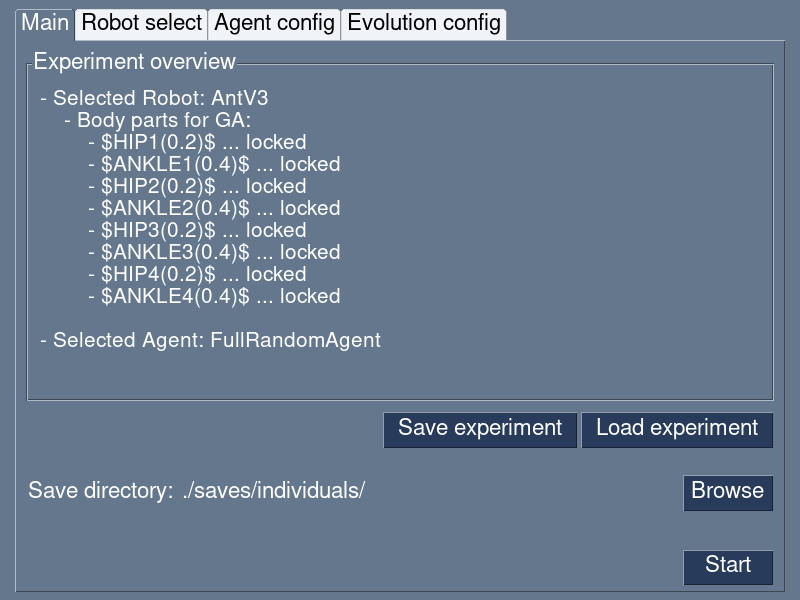
\includegraphics[width=0.6\textwidth]{../img/GUI_main_tab.jpg}
    \caption{Úvodní okno aplikace}
    \label{doc_12_fig:GUI_main}
\end{figure}
Úvodní záložka grafické aplikace (obrázek \ref{doc_12_fig:GUI_main}), ve které
si můžeme prohlédnout zkrácený popis aktuálně nakonfigurované experimentu.
Tento popis je automaticky generován a aktualizovaná tak, aby reflektoval změny
konfigurace daného experimentu. 

Dále pod popisem experimentu najdeme tlačítka pro uložení aktuální konfigurace
a načtení dříve vytvořené konfigurace experimentu. Při ukládání aplikace
vytvoří okno s textovým polem pro pojmenování ukládané konfigurace. Po zvolení
jména je experiment uložen do souboru v pevně zvoleném adresáři. Při načítání
nějakého experimentu aplikace nabídne seznam všech dříve vytvořených
experimentů (jak vytvořených ve zdrojovém kódu, tak v okenní aplikaci), ze
kterého si uživatel může podle jména vybrat (aktuální konfigurace bude bez
možnosti obnovy přepsána).

Úvodní záložka dále nabízí tlačítko \emph{View individual}, které umožňuje v
prohlížeči souborů vybrat uložený záznam nejlepšího jedince z nějakého
předchozího experimentu a toho vizualizovat.

V další řádce se nachází textové pole popisující cílovou cestu, kam bude
uložena složka s daty z konfigurovaného experimentu a tlačítko pro změnu této
cesty.

Poslední je tlačítko \emph{Start}, které okamžitě spustí aktuálně
nakonfigurovaný experiment.

\paragraph{Záložka \emph{Robot select}}
\begin{figure}[!htb]
    \centering
    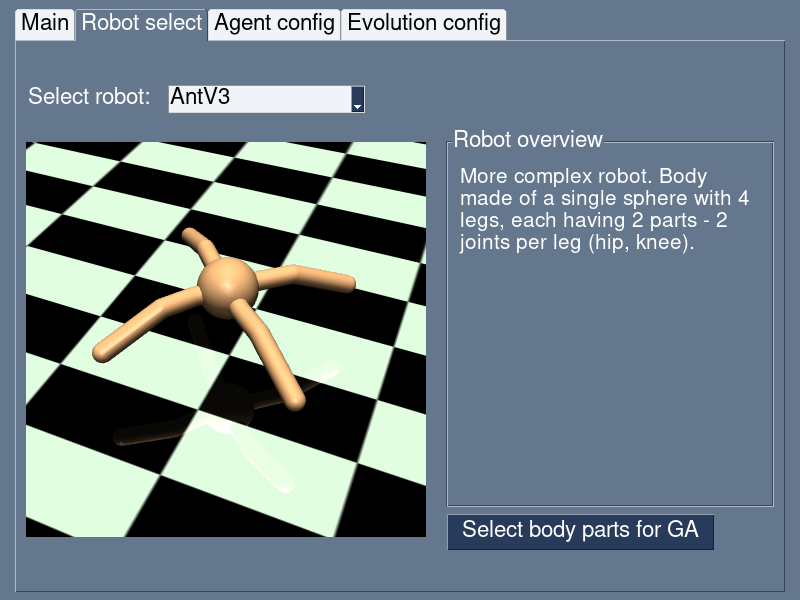
\includegraphics[width=0.6\textwidth]{../img/GUI_robot_tab.jpg}
    \caption{Okno pro volbu robota pro experiment}
    \label{doc_12_fig:GUI_robot}
\end{figure}

Záložka pro výběr robota, který bude využit v konfigurovaném experimentu
(obrázek \ref{doc_12_fig:GUI_robot}), se skládá z rozbalovací nabídky, ve
které~můžeme podle jména zvolit robota. Pro vybraného robota se nám pod
nabídkou ukáže jeho náhledový obrázek a popis. 

Dále se ve spodní části záložky nachází tlačítko \emph{Select body parts for
GA}, které~umožňuje zvolit části těla robota, které se mají v kombinované
evoluci řízení a morfologie vyvíjet. Pokud je toto tlačítko neaktivní, znamená
to, že robot nemá specifikované žádné části těla, které by umožňovali tento
vývoj (více o těchto značkách v kapitole o implementaci v sekci
\ref{imp:robots:symbols}).

\paragraph{Záložka \emph{Agent config}}
\begin{figure}[!htb]
    \centering
    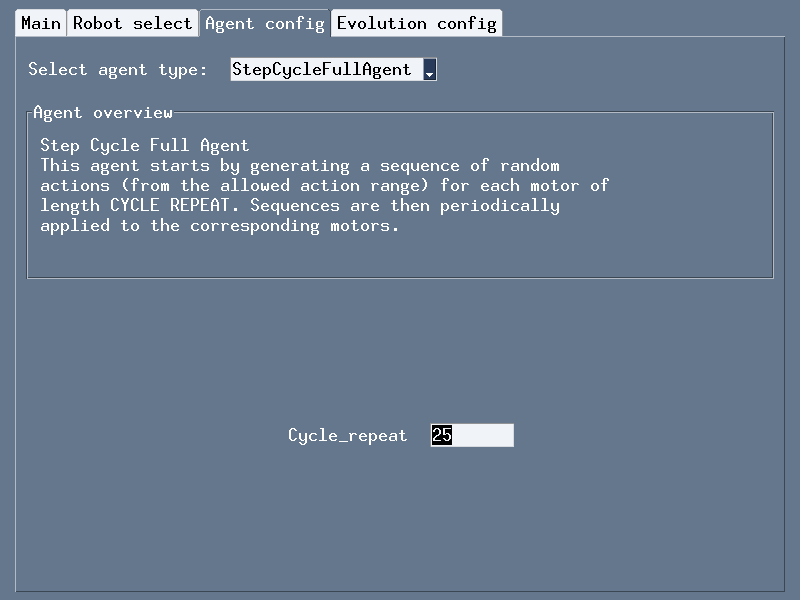
\includegraphics[width=0.6\textwidth]{../img/GUI_agent_tab.jpg}
    \caption{Okno pro volbu agenta pro experiment}
    \label{doc_12_fig:GUI_agent}
\end{figure}
Třetí je záložka pro výběr a konfiguraci agenta (záložka zobrazena na obrázku
\ref{doc_12_fig:GUI_agent}, více o významu a typech evolučních agentů v
kapitole o implementaci v sekci \ref{imp:gaAgents}). V této záložce opět máme
rozbalovací nabídku, pomocí které můžeme vybrat typ agenta. Pod touto nabídkou
se opět nachází popis zvoleného agenta. 

Ve spodní polovině se poté mohou nacházet parametry agenta (specifické pro
každého agenta), které můžeme tímto stylem měnit. V případě nejasnosti o
významu parametru je možné podržet kurzor myši nad názvem daného parametru a
zobrazit tak vysvětlení daného parametru (tato nápověda nemusí být přítomná u
všech parametrů).

\paragraph{Záložka \emph{Evolution config}}
\begin{figure}[!htb]
    \centering
    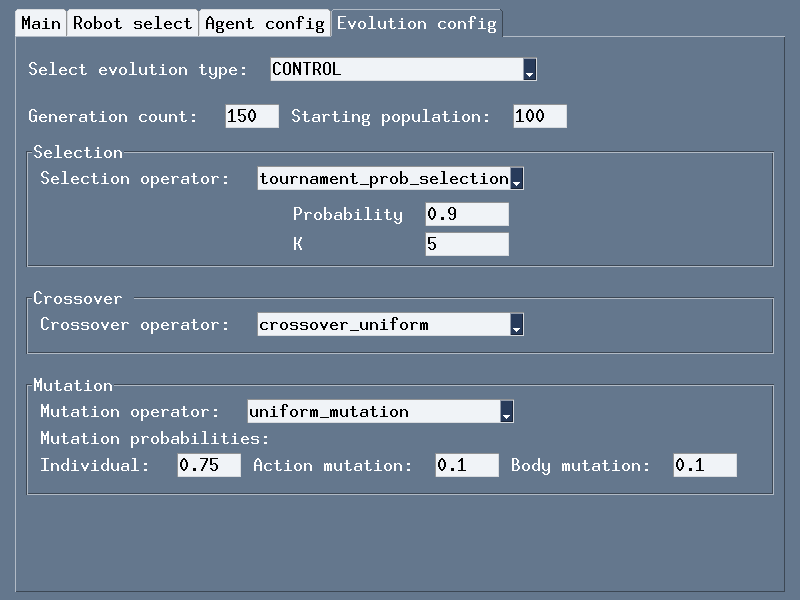
\includegraphics[width=0.6\textwidth]{../img/GUI_evo_tab.jpg}
    \caption{Okno pro úpravu specifických nastavení agenta}
    \label{doc_12_fig:GUI_evo}
\end{figure}

Poslední záložkou (na obrázku \ref{doc_12_fig:GUI_evo}) slouží pro úpravu
samotného evolučního vývoje. Ve vrchní části můžeme vybrat typ evolučního
vývoje. Na výběr máme ze tří možností: 
\begin{itemize}
    \item \texttt{Control} -- vývoj pouze řízení robota,
    \item \texttt{Control-Body parallel} -- současný vývoj řízení i morfologie
        robota,
    \item \texttt{Control-Body serial} -- oddělený vývoj řízení a morfologie
        robota, kde~nejprve proběhne daný počet generací, při kterých bude
        vyvíjeno pouze řízení robota. Následovně se řízení zafixuje a opět po
        stejný počet generací bude vyvíjena pouze morfologie.
\end{itemize}

Dále můžeme zvolit počet generací, kterými evoluce projde a velikost populace
jedinců, na kterých bude vývoj probíhat.

V dalších třech sekcích označených nápisy \emph{Selection}, \emph{Crossover} a
\emph{Mutation}, můžeme měnit samotné genetické operátory pro selekci, křížení
a mutaci jedinců v evolučním algoritmu a upravovat jejich argumenty. Výchozí
hodnoty odpovídají hodnotám specifikovaným ve zdrojovém kódu agentů (popřípadě
se jedná o~hodnoty specifikované načtenou konfigurací experimentu).

\subsection{Textové rozhraní - \emph{TUI.py}} \label{doc_13_TUI}

Textové rozhraní je druhým způsobem, jakým uživatel může pracovat s naší
platformou. Jedná se o částečně omezený přístup v porovnání s grafickým
rozhraním, jelikož textové rozhraní nedovoluje jen za pomocí interakce s
rozhraním vytvářet nové experimenty ani nijak dále konfigurovat ty stávající.

Hodí se hlavně pro spouštění velkých experimentů nebo mnoha experimentů
najednou, u kterých čekáme, že jejich zpracování bude trvat klidně několik
hodin (grafické rozhraní by zpracování experimentů pouze zbytečně zpomalovalo).
Dále se může využívat pro testování nových částí implementace nebo pro zpětnou
vizualizaci výsledků starších experimentů.

\paragraph{Interakce s rozhraním}
Uživatel interaguje s rozhraním z příkazové řádky, pomocí vstupních argumentů,
které zadává při spouštění programu. Seznam a~popis vstupních argumentů
dostupných pro práci s rozhraním společně s příklady využití se nacházejí v
kapitole o implementaci v sekci \ref{imp:TUI}. 

\section{Tvorba, provádění a evaluace experimentů} \label{doc_2_experimenty}

V této části popíšeme způsob, jakým může uživatel pracovat s experimenty, jak
může experimenty vytvářet, spouštět a zpracovávat jejich výsledky.

V podsekci \ref{doc_21_mise_en_place} si představíme jak vytvářet
konfiguraci experiment. Dále v~podsekci \ref{doc_22_cooking} předvedeme
způsoby, jakými spouštět experimenty a v poslední podsekci
\ref{doc_23_seasoning} ukážeme možnosti evaluace výsledků experimentů.

\subsection{Tvorba experimentu} \label{doc_21_mise_en_place}

Pod tvorbou experimentu je myšlena tvorba konfigurace všech částí, ze kterých
se experiment skládá. Toho můžeme docílit dvěma způsoby. 

\paragraph{Tvorba pomocí GUI}
První způsob byl již předveden při představování grafického rozhraní.
Pomocí tohoto rozhraní si uživatel může zcela volně nakonfigurovat všechny
části experimentu -- robota a možnost vyvíjet jeho morfologii, genetického
agenta a jeho parametry a všechny parametry včetně operátorů evolučního
algoritmu. Nakonfigurovaný experiment pak může být pod vlastním jménem uložen,
připraven na spuštění.

\paragraph{Tvorba pomocí kódu}
Uživatel, který by nechtěl pracovat s grafickým rozhraním může místo toho
využít modulu \emph{experiment\_setter.py}, který se nachází v kořenové složce
projektu. Tento modul obsahuje třídu experimentů, obsahující konfigurace všech
experimentů provedených v této práci. Podrobný popis modulu se nachází v
kapitole o implementaci v sekci \ref{imp:experimentsetter}.

Při tvorbě konfigurace experimentu pomocí kódu, musí uživatel vytvořit novou
metodu třídy experimentů, která bude vracet instanci třídy
\texttt{ExperimentParams}, popisující celou konfiguraci experimentu (také
popsána v kapitole o implementaci dříve). Uživatel nakonec dle požadavků modulu
přidá novou metodu do slovníku experimentů, čímž experiment zviditelní navenek.

Tento postup na rozdíl od grafického rozhraní nepovoluje změnu genetických
operátorů jednotlivých agentů ani jednoduchou konfiguraci jednotlivých
parametrů, ale díky blízkosti ke zdrojovému kódu umožňuje uživateli například
podrobněji nahlédnout do způsobu fungování implementace agentů a provádět v
nich změny (kvůli kompatibilitě s původními experimenty musí výchozí agenti
zůstat bez změn -- úpravy ve vlastních kopiích agentů).

\subsection{Spouštění experimentu} \label{doc_22_cooking}

Když je připravená konfigurace experimentu, uživatel má možnost ji vybrat pro
spuštění. Toho opět může být dosaženo dvěma způsoby, které jsme již dříve
popsali a to pomocí grafického, nebo textového rozhraní.

\paragraph{Spouštění s GUI}
Při spouštění experimentu s GUI stačí spustit grafické rozhraní, načíst uložený
experiment a ihned spustit. Hlavní okno aplikace se zamění za běhové okno
experimentu, ve kterém grafické rozhraní zobrazuje základní statistické
hodnoty, ze kterých jde posuzovat průběh experimentu (minimální, průměrná a
maximální fitness populace v každé generaci). 

V grafickém prostředí je experiment vždy spuštěn jen jednou a po definovaném
počtu generací se experiment zastaví a aplikace může být ukončena. Z toho
důvodu se nehodí pro provádění většího množství experimentů.

\paragraph{Spouštění s TUI}
V textovém prostředí je experimenty jednoduché spouštět opakovaně s vícero
nezávislými běhy, které následně mohou být součástí statistického rozboru s
větším množstvím hodnot. Následuje ukázka jak můžeme spustit vlastní
experiment pomocí TUI (z kořenového adresáře projektu).
\begin{code}
./TUI.py --experiment <jmeno_experimentu> --batch 10 --no_graph
\end{code}
Tímto příkazem můžeme spustit libovolný uložený experiment. Celý běh bude 10
krát opakován, kde výsledky jednotlivých nezávislých běhů budou uloženy
společně ve výsledném adresáři (se značkami ve jméně reflektující číslo běhu)
a~v~průběhu evolučního algoritmu nebude generován graf.

\subsection{Evaluace experimentu} \label{doc_23_seasoning}
Evaluace experimentů se může lišit dle typu experimentu a požadavků na jejich
výsledky. Pokud je snaha zjistit, jak dobrý je daný agent, bude~více zajímavé
sledovat průběh fitness hodnot z jednotlivých generací z většího množství
nezávislých běhů stejného experimentu. Naopak, pokud je důležitější jeden
nejlepší výsledek (estetická chůze čtyřnohého robota), bude nás více zajímat
vizualizace samotného výsledku.

\paragraph{Evaluace fitness hodnot krabicovým grafem}
Uživatel má pro evaluaci grafem možnost využít stejného jednoduchého programu,
který byl použit při vykreslování grafů z experimentů pro tuto práci. Tento
program je \emph{plot\_experiment.py} a~nachází se v kořenové složce
tohoto projektu. Tento program přijímá dva vstupní argumenty: 
\begin{itemize}
    \item \texttt{-{}-open} -- povinný argument, po kterém uživatel specifikuje
        cestu ke složce experimentu (běhů experimentu), který chce vykreslit
        uživatel vykreslit,
    \item \texttt{-{}-tick\_step} -- nepovinný argument, po kterém uživatel specifikuje
        celočíselnou hodnotu reprezentující mezery (počet generací) mezi
        vykreslenými záznamy v krabicovém grafu.
\end{itemize}
Po spuštění program vykreslí graf ze zvolených dat. Vysvětlení krabicových
grafů proběhlo v kapitole experimentů v sekci \ref{exp1}.

\paragraph{Vizualizace nejlepších jedinců}
Všechny experimenty vždy ukládají nejlepší vyvinuté jedince. Naše platforma
umožňuje tato data využít k vizualizacím běhů těchto nejlepších jedinců. 

Máme dva způsoby spuštění vizualizací -- pomocí GUI a TUI. Spuštění
vizualizace pomocí obou způsobů bylo již popsáno v předchozích sekcích o
grafickém a textovém rozhraní. 

Vizualizace probíhá ve 3D grafickém prostředí knihovny \emph{MuJoCo}. Ovládací
prvky této aplikace jsou popsány následujícím výčtem.

\begin{itemize}
    \item Pohyb kamery -- pravé tlačítko myši,
    \item Rotace kamery -- levé tlačítko myši,
    \item Přiblížení/oddálení kamery -- kolečko myši,
    \item Zastavení/spuštění simulace -- mezerník,
    \item Posun simulace o jeden krok dále -- šipka vpravo,
    \item Změna kamery -- tabulátor -- každý robot může mít definován různý počet
        kamer (definováno v konfiguračním souboru robota), obvykle má robot
        alespoň jednu kameru, která ho následuje a jednu volnou kameru, se
        kterou může uživatel pohybovat,
    \item Vykreslování každého snímku -- klávesa \texttt{D} -- pokud je tento
        příznak aktivní, není možné zpomalit běh simulace,
    \item Zrychlení/zpomalení běhu simulace -- klávesy \texttt{F} a \texttt{S}
        -- nejdříve je nutné vypnout příznak \emph{vykreslování každého kroku
        simulace},
    \item Vykreslování orientací prostoru každého z kloubů -- klávesa \texttt{E},
    \item Vykreslování kontaktních sil -- klávesa \texttt{C},
    \item Průhledné vykreslování geometrie -- klávesa \texttt{R},
    \item Otevření/zavření nápovědy -- klávesa \texttt{H}.
\end{itemize}
